%----------------------------------------------------------------------------------------
%	PACKAGES AND OTHER DOCUMENT CONFIGURATIONS
%----------------------------------------------------------------------------------------

\documentclass[letterpaper,twoside,11pt]{article}

%% Jose Javier Gonzalez Ortiz %%
%% Plantilla Latex generica   %%
%% 2014-11-08                 %%

\usepackage{lipsum} % Package to generate dummy text throughout this template

\usepackage[sc]{mathpazo} % Use the Palatino font
\usepackage[T1]{fontenc} % Use 8-bit encoding that has 256 glyphs
\linespread{1.05} % Line spacing - Palatino needs more space between lines
\usepackage{microtype} % Slightly tweak font spacing for aesthetics

\usepackage[letterpaper,hmarginratio=1:1,top=32mm,left=20mm,right=20mm,columnsep=20pt]{geometry} % Document margins
\usepackage{multicol} % Used for the two-column layout of the document
\usepackage[hang, small,labelfont=bf,up,textfont=it,up]{caption} % Custom captions under/above floats in tables or figures
\usepackage{booktabs} % Horizontal rules in tables
\usepackage{float} % Required for tables and figures in the multi-column environment - they need to be placed in specific locations with the [H] (e.g. \begin{table}[H])
\usepackage{hyperref} % For hyperlinks in the PDF

\usepackage{lettrine} % The lettrine is the first enlarged letter at the beginning of the text
\usepackage{paralist} % Used for the compactitem environment which makes bullet points with less space between them

\usepackage{abstract} % Allows abstract customization
\renewcommand{\abstractnamefont}{\normalfont\bfseries} % Set the "Abstract" text to bold
\renewcommand{\abstracttextfont}{\normalfont\small\itshape} % Set the abstract itself to small italic text

\usepackage{titlesec} % Allows customization of titles
% \renewcommand\thesection{\Roman{section}} % Roman numerals for the sections
% \renewcommand\thesubsection{\Roman{subsection}} % Roman numerals for subsections
\titleformat{\section}[block]{\large\scshape\centering}{\thesection.}{1em}{} % Change the look of the section titles
\titleformat{\subsection}[block]{\large}{\thesubsection.}{1em}{} % Change the look of the section titles

\usepackage{fancyhdr} % Headers and footers


\usepackage{indentfirst}

% Generic Pakages
    \usepackage[utf8]{inputenc}                         % For Spanish characters
    \usepackage[english]{babel}               % Spanish hyphenation and document rules
    \usepackage{amsmath}                                % Standard math packages
    \usepackage{graphicx}                               % Image insertion.
    \usepackage{tikz}
    \usepackage{caption,subcaption}                     % For custom caption environments

    

    \usepackage{appendix}                               % Enables appendices
    \usepackage{pdfpages}                               % Insert pdfs
    \usepackage{array}                                  % Enables array features
    \usepackage{algorithm}
    \usepackage[noend]{algpseudocode}
    \usepackage{eqparbox}
    \makeatletter
    \def\BState{\State\hskip-\ALG@thistlm}
    \makeatother
    %\usepackage[americanvoltages, europeancurrents, americanresistors, cuteinductors]{circuitikz}                          % Circuit Graphics
    \usepackage{mathtools}
    \usepackage{amsthm}
    
%Additional Features
    
    \usepackage{enumerate}                              % Custom numerate, useful for i,ii,iii... I,II,III...
    \usepackage{sectsty}                                % Allows customizing section commands
    \usepackage{todonotes}                              % useful for leaving todonotes
    \usepackage[space]{grffile}                         % insert files with spaces
     %\usepackage{microtype}                             % Beatify engine
    %\usepackage[superscript]{cite}                     % CIting with superscript numerals
    %\usepackage{xcolor}                                    % Required for inserting color
    %\usepackage[usenames,dvipsnames]{color}                % Required for custom colors
    %\usepackage{xargs}                                 % Expanded arguments features
    %\usepackage{fix-cm}                                 % Computer-Modern at arbitrarysizes
    \usepackage{siunitx}                               % For SI Units
    %\usepackage{eurosym}                                % Eurosymbol
    %\usepackage{pdflscape}                              % enables landscape for pdfs
    %\usepackage{longtable}                              % Tables than span multipages

% Custom Settings
    % \decimalpoint                                       % American Decimal Point instead of Spanish comma

    % Margins
    %     \topmargin      = -0.45in
    %     \evensidemargin = 0in
    %     \oddsidemargin  = 0in
    %     \textwidth      = 6.5in
    %     \textheight     = 9.0in
    %     \headsep        = 0.25in

    % \pagestyle{fancy}
    % \lhead{\HWAuthorName}
    % \chead{}
    % \rhead{\HWClass : \HWTitle}
    % \lfoot{}
    % \cfoot{\thepage}
    % \rfoot{}
    
    % \renewcommand\headrulewidth{0.4pt} % Size of the header rule
    % \renewcommand\footrulewidth{0.4pt} % Size of the footer rule

    \numberwithin{equation}{section} % Number equations within sections (i.e. 1.1, 1.2, 2.1, 2.2 instead of 1, 2, 3, 4)
    \numberwithin{figure}{section} % Number figures within sections (i.e. 1.1, 1.2, 2.1, 2.2 instead of 1, 2, 3, 4)
    \numberwithin{table}{section} % Number tables within sections (i.e. 1.1, 1.2, 2.1, 2.2 instead of 1, 2, 3, 4)

    \renewcommand{\labelitemi}{$\bullet$}                       %%bullet1 circle
    \renewcommand{\labelitemii}{\leavevmode \hbox to
    1.2ex {\hss \vrule height .9ex width .7ex depth -.2ex\hss }} %%bullet2 box

    \newcommand{\ul}[1]        {\underline{\smash{#1}}}         %%closer underline
    \newcommand{\gm}[1]         {\guillemotleft #1\guillemotright}  %$ pretty <<sth>>$

    \DeclarePairedDelimiter\floor{\lfloor}{\rfloor}
    \DeclarePairedDelimiter\ceil{\lceil}{\rceil}

%%%%%%%%%%%%%%%%%%%%%%%%%%%%%%%%%%%%%%%%%%%%%%%%%%%%%%%%%%%%%%%%%%%%%%%%%%%%%%%%%%
%%%                             CODIGO                                         %%%
%%%%%%%%%%%%%%%%%%%%%%%%%%%%%%%%%%%%%%%%%%%%%%%%%%%%%%%%%%%%%%%%%%%%%%%%%%%%%%%%%%

% Code insertion
    \usepackage{listings}                               % Main package for inserting code
    \usepackage{courier}                                % For using the courier font

    \AtBeginDocument{\numberwithin{lstlisting}{section}}  % Number listings within sections (i.e. 1.1, 1.2, 2.1, 2.2 instead of 1, 2, 3, 4)
    
    %%\captionsetup[lstlisting]{font={small,tt}}            %  Listings Font Size
    
    % \renewcommand{\lstlistingname}{Código}              % For Codigo caption (requires caption package)

    \definecolor{background}{gray}{.98}                 % Background color definition
    \definecolor{comments}{RGB}{51,102,0}               % Comments   color definition
    \definecolor{keywords}{RGB}{0,0,120}                % Keywords   color definition
    \definecolor{keywords2}{RGB}{204,0,102}             % Keywords2  color definition
    \definecolor{numbers}{RGB}{127, 0, 127}             % Keywords2  color definition

    \definecolor{Maroon}{RGB}{128, 0, 0}

       % morekeywords={add,sub,mul,mulu,nand,sll,sra,srl,sltu,addi,sw,lw,beq,jarl,lui},
    \lstdefinelanguage{ICAI-RiSC-16}
   {morekeywords={add,sub,mul,mulu,nand,sll,sra,srl,sltu,addi,sw,lw,beq,jalr,lui,la,med},
        sensitive=false,
        morecomment=[l]{\#},
        morecomment=[l][\color{Maroon}]{.},
        morekeywords=[2]{r0, r1, r2, r3, r4, r5, r6, r7},
        keywordstyle=[2]{\color{violet}},
        % literate=%
        %    *{0}{{{\color{red!20!violet}0}}}1
        %     {1}{{{\color{red!20!violet}1}}}1
        %     {2}{{{\color{red!20!violet}2}}}1
        %     {3}{{{\color{red!20!violet}3}}}1
        %     {4}{{{\color{red!20!violet}4}}}1
        %     {5}{{{\color{red!20!violet}5}}}1
        %     {6}{{{\color{red!20!violet}6}}}1
        %     {7}{{{\color{red!20!violet}7}}}1
        %     {8}{{{\color{red!20!violet}8}}}1
        %     {9}{{{\color{red!20!violet}9}}}1
        %morecomment=[s]{/*}{*/},
        %morestring=[b]"
    }


    \lstset{
        frame=Ltb,
        framerule=0pt,
        aboveskip=0.5cm,
        framextopmargin=3pt,
        framexbottommargin=3pt,
        framexleftmargin=0.4cm,
        framesep=0pt,
        rulesep=.4pt,
        backgroundcolor=\color{background},
        rulesepcolor=\color{black},
        rulecolor=\color{black},
        %
        stringstyle=\ttfamily,
        basicstyle=\small\ttfamily,
        commentstyle=\itshape\color{comments},
        keywordstyle=\bfseries\color{keywords},
        %
        numberstyle=\tiny,
        numbers=left,
        numbersep=15pt,
        numberfirstline = false,
        %
        breakatwhitespace=false,         % sets if automatic breaks should only happenat whitespace
        breaklines=true,                 % sets automatic line breaking
        captionpos=b,                    % sets the caption-position to bottom
        escapeinside={<@}{@>},            % if you want to add LaTeX within your code
        keepspaces=true,                 % keeps spaces in text, useful for keepingindentation of code (possibly needs columns=flexible)
        showspaces=false,                % show spaces everywhere adding particularunderscores; it overrides 'showstringspaces'
        showstringspaces=false,          % underline spaces within strings only
        showtabs=false,                  % show tabs within strings adding particularunderscores
        stepnumber=1,                    % the step between two line-numbers. If it's1, each line will be numbered
        tabsize=2,                       % sets default tabsize to 2 spaces
    }
    

    \lstdefinestyle{customvhdl}{
        language=vhdl,                              % Language
        morekeywords = {},
        morestring=[b][\color{numbers}]',
        morestring=[b][\color{numbers}]",
        emph={std_logic,std_logic_vector,integer,unsigned,to_unsigned},
        emphstyle={\color{keywords2}\bfseries},%
        %deletekeywords={...},            % if you want to delete keywords from the given language
    }

    \lstdefinestyle{customcpp}{
        language = C++,
       %  directivestyle={\color{black}}
       % emph={int,char,double,float,unsigned},
       % emphstyle={\color{blue}}
    }

    \lstset{style = customcpp}



    % Grey scale definitions - Printing
    %\definecolor{background}{gray}{.98}
    %\definecolor{comments}{gray}{.45}
    %\definecolor{keywords}{gray}{.25}


%%%%%%%%%%%%%%%%%%%%%%%%%%%%%%%%%%%%%%%%%%%%%%%%%%%%%%%%%%%%%%%%%%%%%%%%
%%%%%%%%%%%%%%%%%%%%%%       HERE BE DRAGONS        %%%%%%%%%%%%%%%%%%%%
%%%%%%%%%%%%%%%%%%%%%%%%%%%%%%%%%%%%%%%%%%%%%%%%%%%%%%%%%%%%%%%%%%%%%%%%
%
%%%%%%%%%%%%%%%%%%%%%%%%%%%%%%%%%%%%%%%%%%%%%%%%%%%%%%%%%%%%%%%%%%%%%%%%
%%%% Paragraph separation
%\setlength{\parskip}{.5em}
%%%%%%%%%%%%%%%%%%%%%%%%%%%%%%%%%%%%%%%%%%%%%%%%%%%%%%%%%%%%%%%%%%%%%%%%
%%%% Table separation
%\renewcommand{\arraystretch}{1.3}
%%%%%%%%%%%%%%%%%%%%%%%%%%%%%%%%%%%%%%%%%%%%%%%%%%%%%%%%%%%%%%%%%%%%%%%%
%%%% 9+ Arguments functions
%\newcommand{\function}[9]{%
%        \def\tempa{#1}%
%        \def\tempb{#2}%
%        \def\tempc{#3}%
%        \def\tempd{#4}%
%        \def\tempe{#5}%
%        \def\tempf{#6}%
%        \def\tempg{#7}%
%        \def\temph{#8}%
%        \def\tempi{#9}%
%        \functioncont
%    }
%%%%%%%%%%%%%%%%%%%%%%%%%%%%%%%%%%%%%%%%%%%%%%%%%%%%%%%%%%%%%%%%%%%%%%%%
%%%% Rules for longtable
%\newcommand{\mytoprule}{\specialrule{1.5pt}{0em}{0em}}
%\newcommand{\mymidrule}{\specialrule{.75pt}{0em}{0em}}
%\newcommand{\mybottomrule}{\specialrule{1.5pt}{0em}{0em}}
%
%%%%%%%%%%%%%%%%%%%%%%%%%%%%%%%%%%%%%%%%%%%%%%%%%%%%%%%%%%%%%%%%%%%%%%%%
%%%% Roman numerals at the start
%
%\pagenumbering{roman}
%\tableofcontents
%\newpage
%\listoftables
%\newpage
%\pagenumbering{arabic}
%%%%%%%%%%%%%%%%%%%%%%%%%%%%%%%%%%%%%%%%%%%%%%%%%%%%%%%%%%%%%%%%%%%%%%%%
%%%% More than 18 floating figures/tables - force to put
%\clearpage
%%%%%%%%%%%%%%%%%%%%%%%%%%%%%%%%%%%%%%%%%%%%%%%%%%%%%%%%%%%%%%%%%%%%%%%%
%%%% Landscape tables recommendations
%\topmargin      = -0.95in
%\evensidemargin = 0in
%\oddsidemargin  = 0in
%\textwidth      = 6.5in %6.5in
%\textheight     = 9.75in
%\headsep        = 0.25in
%\small  % Switch from 12pt to 11pt
%\setlength\LTleft{0pt}            % default: \parindent
%\setlength\LTright{0pt}           % default: \fill
%%%%%%%%%%%%%%%%%%%%%%%%%%%%%%%%%%%%%%%%%%%%%%%%%%%%%%%%%%%%%%%%%%%%%%%%
%%%% Bold columns table
%>{\bfseries\arraybackslash}m{1.1in}
%
%%%%%%%%%%%%%%%%%%%%%%%%%%%%%%%%%%%%%%%%%%%%%%%%%%%%%%%%%%%%%%%%%%%%%%%%
%%%% \epigraph{}
%
%\makeatletter
%\patchcmd{\epigraph}{\@epitext{#1}}{\itshape\@epitext{#1}}{}{}
%\makeatother
%%%%%%%%%%%%%%%%%%%%%%%%%%%%%%%%%%%%%%%%%%%%%%%%%%%%%%%%%%%%%%%%%%%%%%%%
%%%% Quotes -> chapquote enviroment
%\makeatletter
%\newenvironment{chapquote}[2][2em]
%  {\setlength{\@tempdima}{#1}%
%   \def\chapquote@author{#2}%
%   \parshape 1 \@tempdima \dimexpr\textwidth-2\@tempdima\relax%
%   \itshape}
%  {\par\normalfont\hfill--\ \chapquote@author\hspace*{\@tempdima}\par\bigskip}
%\makeatother
%%%%%%%%%%%%%%%%%%%%%%%%%%%%%%%%%%%%%%%%%%%%%%%%%%%%%%%%%%%%%%%%%%%%%%%%

\pagestyle{fancy} % All pages have headers and footers
\fancyhead{} % Blank out the default header
\fancyfoot{} % Blank out the default footer
\fancyhead[L]{Jose Javier Gonzalez Ortiz}
\fancyhead[R]{EECS 587 : Parallel Computing} % Custom header text
\fancyfoot[RO,LE]{\thepage} % Custom footer text


\setlength{\parskip}{2mm}
\setlength{\headheight}{13.6pt}
%----------------------------------------------------------------------------------------
%	TITLE SECTION
%----------------------------------------------------------------------------------------

\title{\vspace{-15mm}\fontsize{24pt}{10pt}\selectfont\textbf{Parallel Implementation of Multiple Interdependent Lindenmayer Systems}} % Article title

\author{
\large
\textsc{Jose Javier Gonzalez Ortiz}\thanks{\href{mailto:jjgo@umich.edu}{jjgo@umich.edu}}\\[2mm] % Your name
\normalsize University of Michigan \\ % Your institution
% \normalsize \href{mailto:jjgo@umich.edu}{jjgo@umich.edu} % Your email address
% \vspace{-5mm}
}
\date{\today}

%----------------------------------------------------------------------------------------

\begin{document}

\maketitle % Insert title

\thispagestyle{fancy} % All pages have headers and footers

%----------------------------------------------------------------------------------------
%	ABSTRACT
%----------------------------------------------------------------------------------------

\begin{abstract}

\noindent \lipsum[1] % Dummy abstract text

\end{abstract}

%----------------------------------------------------------------------------------------
%	ARTICLE CONTENTS
%----------------------------------------------------------------------------------------

\begin{multicols}{2} % Two-column layout throughout the main article text

\section{Introduction}
% \vspace{-6mm}
\lettrine[nindent=0em,lines=2]{M}
odern techniques for botanic and arboreal growth simulation rely in specific and dedicated models to correctly recreate the behavior of different types of plants. This creates a segmented and disconnected variety of models and techniques. As A. Lindenmayer and Przemyslaw described in \cite{Prusinkiewicz:1996:ABP:235579}, almost all botanical structures can be successfully model by Lindenmayer Systems.

However, raw L-Systems are not complex enough for this task and therefore we need to include both a parametric implementation to successfully model these types of structures. Moreover, parametric L-Systems in spite of depending on a number of initial parameters and conditions, they are deterministic. To cope with this limitation, we introduce randomness in the traditional form described in \cite{Prusinkiewicz:1996:ABP:235579}, by using Stochastic-Parametric L-Systems. This systems will have production rules that will not only rely on several parameters to correctly scalate the complexity of the system but will also apply this rules using a source of randomness to choose between a number of specified rules.

Another aspect we have to properly take into a account is the fact that botanical growth almost never occurs in a isolated fashion, and therefore we will be interested in looking at a framework that can accommodate the simultaneous derivation of multiple L-Systems. Having multiple stochastic L-Systems produces a non-realistic result as we will see later, so to compensate for this caveat we had to define the concept of Interdependent L-System.

In this paper we investigate the use of Interdependent L-System to realistically model the growth of a forest and we analyze several parallel implementations of this problem in a shared memory machine using OpenMP. L-Systems are parallel rewriting grammar which initially would seem to simplify the problem, but this derivation step leads to highly uneven amounts of work in a great number of scenarios. Furthermore, as we shall see later, adding the interdependence to the systems serializes the problem since after every timestep each system will need to communicate a number of metric to a variable number of other systems. This problem will produce a scenario experienced by a great amount of local simulation techniques.

We will introduce several parallel algorithms with increasing complexity and with increasing speedup and compare their behavior under different types of datasets, which from a simulation perspective would translate into different ecosystems. The final algorithm will involve calculating the connected components of the forest graph to initially subdivide the problem in equally complex albeit not equally balanced subproblems, and introduce a general approach to tackle this subproblems. To accomplish this, the algorithm will deserialize the time dimension by allowing some L-Systems to carry out further iterations as long as the correctness constraints are met. We will also analyze the bigger bottleneck of the algorithm and the way it tries to cope with the variability of input systems.

\textbf{Overview:} First  we will start by providing a background in canonical, parametric and stochastic L-Systems in Section \ref{sec:background}. Section \ref{sec:interdependence} will elaborate the model used to realistically model the problem and will discuss the serial implementation that was carried out. The parallel algorithms designed to solve this problem are discussed in Section \ref{sec:parallelization} and their associated results are shown in Section \ref{sec:results} and analyzed in Section \ref{sec:discussion}.

\subsection{Previous Work} % (fold)
\label{sub:previous_work}
\textbf{General L-Systems:} Prusinkiewicz and Lindenmayer gave the basic definition to the L-System algorithm and structure in \cite{Prusinkiewicz:1996:ABP:235579}. This was further extended by the work carried out in \cite{Parish:2001:PMC:383259.383292,Prusinkiewicz:1994:ST:192161.192254,Prusinkiewicz:2001:UPI:383259.383291}

\textbf{Parallelizing L-Systems:} Lacz and Hart introduced the use of manually written pixel shaders to compute L-Systems \cite{Lacz04proceduralgeometry}. A distributed memory approach making use up to 8 CPUs and the Message Passing Interface (MPI) was described in \cite{4392608}. An algorithm form the Parallel Generation of L-Systems was introduced by \cite{LIPP-2009-PGL}. The approach was appropriate for both GPU and multi-core CPUs, parallelizing both the derivation and interpretation of given L-Systems. The implementation provided was generic and supported parametric, stochastic and context sensitive productions. The work was further extended in \cite{LIPP-2010-PGMS} to make the algorithm work with multiple L-Systems.

\textbf{Forest Simulation:} L-Systems are within the most popular grammars to satisfactory model botanical structures. The definitions introduced by \cite{Prusinkiewicz:1996:ABP:235579} were later improved to more realistic three dimensional trees for \cite{4055766}. Since then, both models have been used in a number of forest growth models.

The model proposed by \cite{KurthSloboda2002} provides a wonderful framework to model the interdependence of L-Systems. Geometrical interpretation of parameters was used to calculate shadow cones and a carbon allocation economy was used to successfully control the growth of the trees. A later paper introduced a quasi-physical simulation of large-scale dynamic forest scenes by introducing a similar growth model and a wind field to account for environmental factors. Finally, \cite{Runions07modelingtrees} introduced a new model by employing a three dimensional version of the space colonization algorithm.
% subsection previous_work (end)

%------------------------------------------------

\section{Background} % (fold)
\label{sec:background}

\subsection{Definition} % (fold)
\label{sub:definition}

The work presented in this paper is based on L-systems so we will briefly introduce this modeling structure.

\emph{L-Systems:} are parallel rewriting systems and a type of formal grammar. L-systems are now commonly referred as \emph{parametric} L-systems, defined as a tuple:
\begin{equation}
	\textbf{G} = (V, \omega, P)
\end{equation}
where
\begin{compactitem}
\item $\textbf{V}$ (\emph{alphabet}) is a set of symbols containing the elements in the string that can be replaced
\item $\boldsymbol\omega$ (\emph{axiom}) is a string of symbols from $V$ defining the initial state of the system.
\item $\textbf{P}$ is a set of \emph{production rules} which define the way variables can be replaced with combinations of constants and variables. Each rule is composed by a \emph{predecessor} and a \emph{successor}. The successor will consist of a list of symbols that will replace the predecessor. Usually the predecessor contains only one symbol, if it involves more, the system is called \emph{context sensitive}. If a production rule is not specified for a symbol, the identity production is assumed.
\end{compactitem}

\emph{Parametric L-systems:} We can further expand the definition of L-system to accommodate parameters. In a parametric grammar, each symbol in the alphabet has a list of parameters associated with it. Parameters are usually real valued but there is not constraint in the mathematical structures that can be used. Production rules need to be extended to deal with parametric symbols. Parameters can be both \emph{global} or \emph{local} depending on if they belong to the current predecessor. Parameters are used in both conditional statements to choose between different production rules and for modifuying the parameters of the symbols in the successor. In the following example \eqref{eq:example}, we can see the behavior, where $g$ is a global parameter.
\begin{equation}
\label{eq:example}
	A(x,y) : x < 2 \quad\rightarrow\quad A(g,x+1) C B(3,y)
\end{equation}

\emph{Stochastic L-systems:} In order to deal with non-deterministic models, randomness can be introduced in the model by defining for each production rule $p \in P$ a set of production rules $\overline{p} = \{p_1,p_2\ldots p_k\}$ with associated probabilities $\overline{q} = \{q_1,q_2\ldots q_k\}$ and a random variable $R$ that will evaluate the rule $p$ as $p_i$ with probability $q_i$. This kind of grammars are tremendously useful when generating great amounts of L-systems, because otherwise all the elements in the group would look the same.

% subsection definition (end)

\subsection{Application} % (fold)
\label{sub:application}

Once defined the specific type of grammar or combination of grammars, to actually generate the geometry described by a L-System we have to execute two stages: the \emph{derivation} of the final symbol string and the \emph{interpretation} of such string to a particular geometry or structure.

\textbf{Derivation:} this phase involves a number of successive interpretation iterations. In each iteration, all symbols in the current state are translated in parallel using the production rules. For each symbol, a production rule with a matching predecessor and condition is searched. Once found, the symbol will be substituted by the parametric symbols in the successor which are evaluated using the global parameters at the current iteration and the local parameters of the symbol that is being substituted. The initial state is the axiom of the system, the state string is updated after each iteration, so the final state is specified by the arbitrary number $k$ of iterations that we have defined.
\vfill
\columnbreak
\textbf{Interpretation:} after the final state string of symbols is produced a set of interpretation rules will have to be applied to extract the information of the system. Most commonly, a geometric representation is generated by using two or three dimensional Turtle Geometry \cite{abelson1986turtle}. This translates the commands into modifications of the turtle state, which is represented by a position in space and a angle orientation in such space. Usually most modifications can be associated with euclidian affine transformation. However \emph{branching} (or \emph{bracketed}) systems will also use push and pop commands to input the current \emph{turtle state} into a stack for later recovery.
% subsection application (end)
% section background (end)

\begin{figure}[H]
  \centering
  \begin{subfigure}{.5\textwidth}
    \centering
    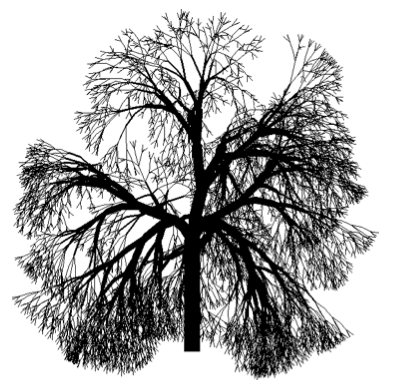
\includegraphics[width=.63\textwidth]{trees1.png}
    \caption{}
    % \label{fig:balanced}
  \end{subfigure}%
\end{figure}
\begin{figure}[H]
\ContinuedFloat
  \begin{subfigure}{.5\textwidth}
    \centering
    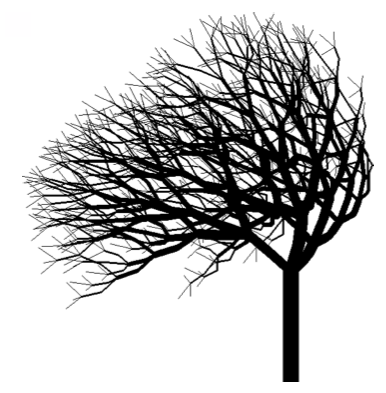
\includegraphics[width=.63\textwidth]{trees2.png}
    \caption{}
    % \label{fig:unbalanced}
  \end{subfigure}
  \caption{Examples of trees with ternary branching$^{\text{\cite{Prusinkiewicz:1996:ABP:235579}}}$}
   \label{fig:ttrees}\end{figure}

\section{Interdependence} % (fold)

\label{sec:interdependence}

Three dimensional parametric and stochastic L-Systems are a really powerful tool that help us model complex botanical structures such as monopodial, sympodial and ternary trees.By varying global parameters we can regulate some fixed parameters such as the way gravity affects the tree or the branching angle that the tree will follow. We can visualize these ideas in the ternary trees shown in Figure \ref{fig:ttrees}.

However, whereas we need stochastic systems as a source of variability to realistically emulate the structure of forests, there is a enormous caveat using them for multiple independent L-systems. To look into the problem lets consider the size of a state string $S$ as $|S| = L$. If each production rule translate one symbol into two and we only have deterministic production rules, the output will have size $2L$. However, if each production rule only substitutes with a $50\%$ chance then we only expect half of the symbols to change and the expected size of the output string will be $3L/2$. So we can find a proportionality between input and output sizes and this will deem an exponential growth. However, if by chance, one string gets a significantly greater or lower amount of successful production rules this will affect in the next iteration, since having more symbols in the string will allow the system to grow faster and viceversa.

This produces an oddly looking unrealistic system as we can see in Figure \ref{fig:stochas} where one of the plants has, after a few iterations grown bigger, and will keep doing so; whereas other plants have carried average iterations resulting in similar systems. This phenomenon can be justified by the fact that: a) the systems are completely independent of each other and therefore do not share any common parameters, b) we are not taking into account any real model for the shared medium, such as mineral resources.

\begin{figure}[H]
  % \centering
    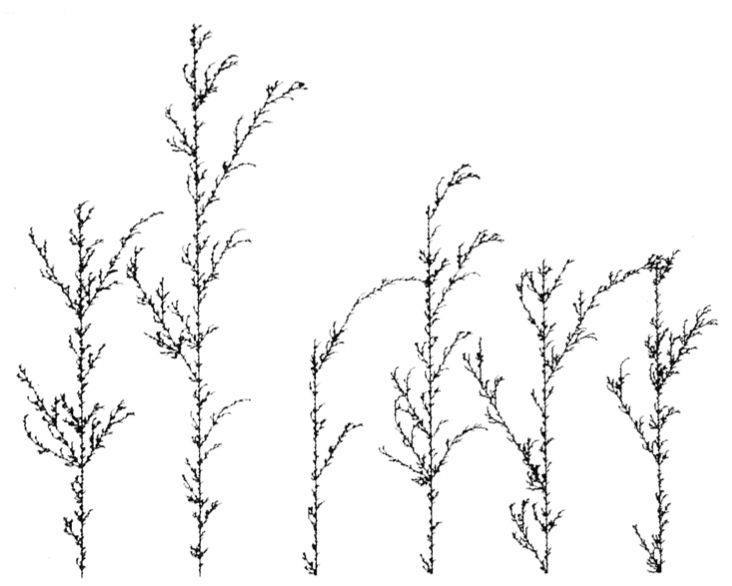
\includegraphics[width=.5\textwidth]{stochastic.png}
    \caption{Simulated growth of several simple stochastic L-Systems$^{\text{\cite{Prusinkiewicz:1996:ABP:235579}}}$}
    \label{fig:stochas}
\end{figure}

In a similar fashion as \cite{KurthSloboda2002} did, we can employ  both the global parameters to the system and universal parameters to the whole group of systems to thwart this undesired behavior. These parameters display the relationship between different systems or different parts of the same system, and are usually updated after each derivation step with the information provided by different metrics on the current string state.  Depending on the locality of the parameters we can differentiate two types of dependence:
\begin{compactenum}[a)]
\item \textbf{Selfdependence} - In this case there exists a relationship between different parts of the same system. For example, given a tree whose production rules depend on the amount of light received by each branch would need to update this information after each timestep considering the shadows projected by its own branches.
\item \textbf{Interdependence} - A more complex case that involves relationships between potentially different types of L-Systems, and that reflects a reciprocal interaction between them. We can extend the previous example, given a number of trees if we consider not only the shadow of a tree to itself, but the shadow projected from other trees we will have introduced a interdependence relationship into the growth simulation.
\end{compactenum}

 Independent and selfdependent systems provide a embarrassingly parallel problem, since each system can be analyzed without considering the others they can be treated as individual problems. The load balancing can achieved by a simple manager-worker scheme using a shared queue. However, interdependent groups of L-Systems can pose a nontrivial parallelization given appropriate constraints. For this paper we have used a local resource economy which translates in the following behavior. A tree will only be affected by the trees within a radius R, which from now onwards will referred to as his \emph{neighbors}. If a tree is bigger than the average size of their neighbors then it will be harder for it to grow at the next iteration, preventing the overgrowth behavior depicted in Figure \ref{fig:stochas}. If a tree is smaller than the average size of its neighbors, then it will more likely for it to grow in the next iteration, compensating the randomness in previous iterations. We need to use this constraints since as we explained before, whereas randomness is a good source of variability for the population, it deeply alters the growth rate of different systems leading to undesired and unrealistic behaviors.

 We still need to define what the \emph{size} of a tree means from an analytical viewpoint. We will use the concept of \emph{metrics}, functions when given as an input a list of parametric symbols, output a list of real valued parameters that reflect different aspects of the system. In our implementation the metric employed measured both the number of nodes (points where branching occurs) and leaves (terminal points of the system) to account for the dimensions of the tree.
\vfill
\columnbreak
 A serial implementation of the described scenario was carried out\footnotemark. A fixed number of different L-Systems composed a given probability distribution of monopodial, sympodial and ternary trees was randomly distributed in a square surface. All these tree systems where slightly modified from the Honda canonical definitions given in \cite{Prusinkiewicz:1996:ABP:235579} to accommodate for randomness in the growth. Next, a neighbor look-up list was initialized, since neighboring relations do not change throughout the simulation. For a fixed number $k$ of iterations, each system was applied the derivation procedure and its metric recalculated and stored in a global array. Then, before starting the next iteration, the growth parameter of each system was updated using the metrics from its neighbors.

 This implementation allows for huge variability of environments. Modifying the probability distribution of trees, the size of the Area, the number of systems and the number of iterations allow us to model from old, dense boreal forests to a widely spaced savanna.

\footnotetext{All the code for this project can be found in \href{http://github.com/JJGO/Parallel-LSystem}{http://github.com/JJGO/Parallel-LSystem}}

% section interdependence (end)

\section{Parallelization} % (fold)
\label{sec:parallelization}

When looking at a decently sized forest ($N \approx 100$) and a considerable number of iterations ($k \approx 14$), the serial implementation starts taking seconds on most modern machines. Trying to increase any of the parameters goes to the domain of minutes and even hours. Therefore, the problem can use parallelization techniques in order to reduce the computation time by introducing more processing power. For this analysis we have chosen a shared memory architecture using the OpenMP application programming interface in C++. In this paper we are going to focus in the parallelization of the derivation step for the interdependant system described in Section \ref{sec:interdependence}. \phantom{This is}

The interpretation step of multiple L-Systems is an inherently embarrassingly parallel problem since all of the systems are independent when it comes to interpretation. To further optimize the parallelization of the interpretation step, one can look at parallelizing the interpretation of an individual L-System. This can be easily done for \emph{non-branching} systems by replacing each symbol with its associated affine transformation (4x4 matrix). Since matrix multiplication is an associative operation we can easily solve the problem by using a \emph{reduce} function. \emph{Branching} systems can follow a similar approach but the complexity escapes the scope of the current paper. A more  detailed explanation can be found in \cite{LIPP-2010-PGMS}.

\subsection{Naive parallelization} % (fold)
\label{sub:naive_parallelization}

A initial naive parallelization can be used by just simply parallelizing each one of the derivation iteration steps. Using a dynamic scheduling algorithm, the different processor will evenly split the work and solve each iteration in parallel. As we shall see later in Section \ref{sec:results}, this approach decreases the overall time but is far from perfect. The main disadvantage associated with this approach comes from the fact that a barrier must be set up at the end of each iteration to ensure correctness. This will imply that for $p$ processors and $N$ similarly sized trees, at the end of each iteration approximately $r \equiv N \mod p$ processors will be still working and $N - r$ will be idle, waiting for the rest to finish and wasting processing power.

% subsection naive_parallelization (end)

% section parallelization (end)

\section{Results} % (fold)
\label{sec:results}

% section results (end)

\section{Discussion} % (fold)
\label{sec:discussion}

% section discussion (end)

\section{Conclusion} % (fold)
\label{sec:conclusion}

% section conclusion (end)


%----------------------------------------------------------------------------------------
%	REFERENCE LIST
%----------------------------------------------------------------------------------------
\nocite{*}
\bibliographystyle{alpha}
\bibliography{mybib}
% \begin{thebibliography}{99} % Bibliography - this is intentionally simple in this template

% \bibitem[Figueredo and Wolf, 2009]{Figueredo:2009dg}
% Figueredo, A.~J. and Wolf, P. S.~A. (2009).
% \newblock Assortative pairing and life history strategy - a cross-cultural
%   study.
% \newblock {\em Human Nature}, 20:317--330.
 
% \end{thebibliography}

%----------------------------------------------------------------------------------------

\end{multicols}

\end{document}
